\documentclass{article}
\usepackage {inputenc, fullpage, listings, amsmath, graphicx, amssymb, xcolor}

\parindent 0pt

\title{%
   ECE 260: Continuous-Time Signals and Systems\\
    Assignment 3A\\
    }
\date{}

\begin{document}

\maketitle

4.1 {\bf [compute convolution]}\\
(e)
\begin{center}
    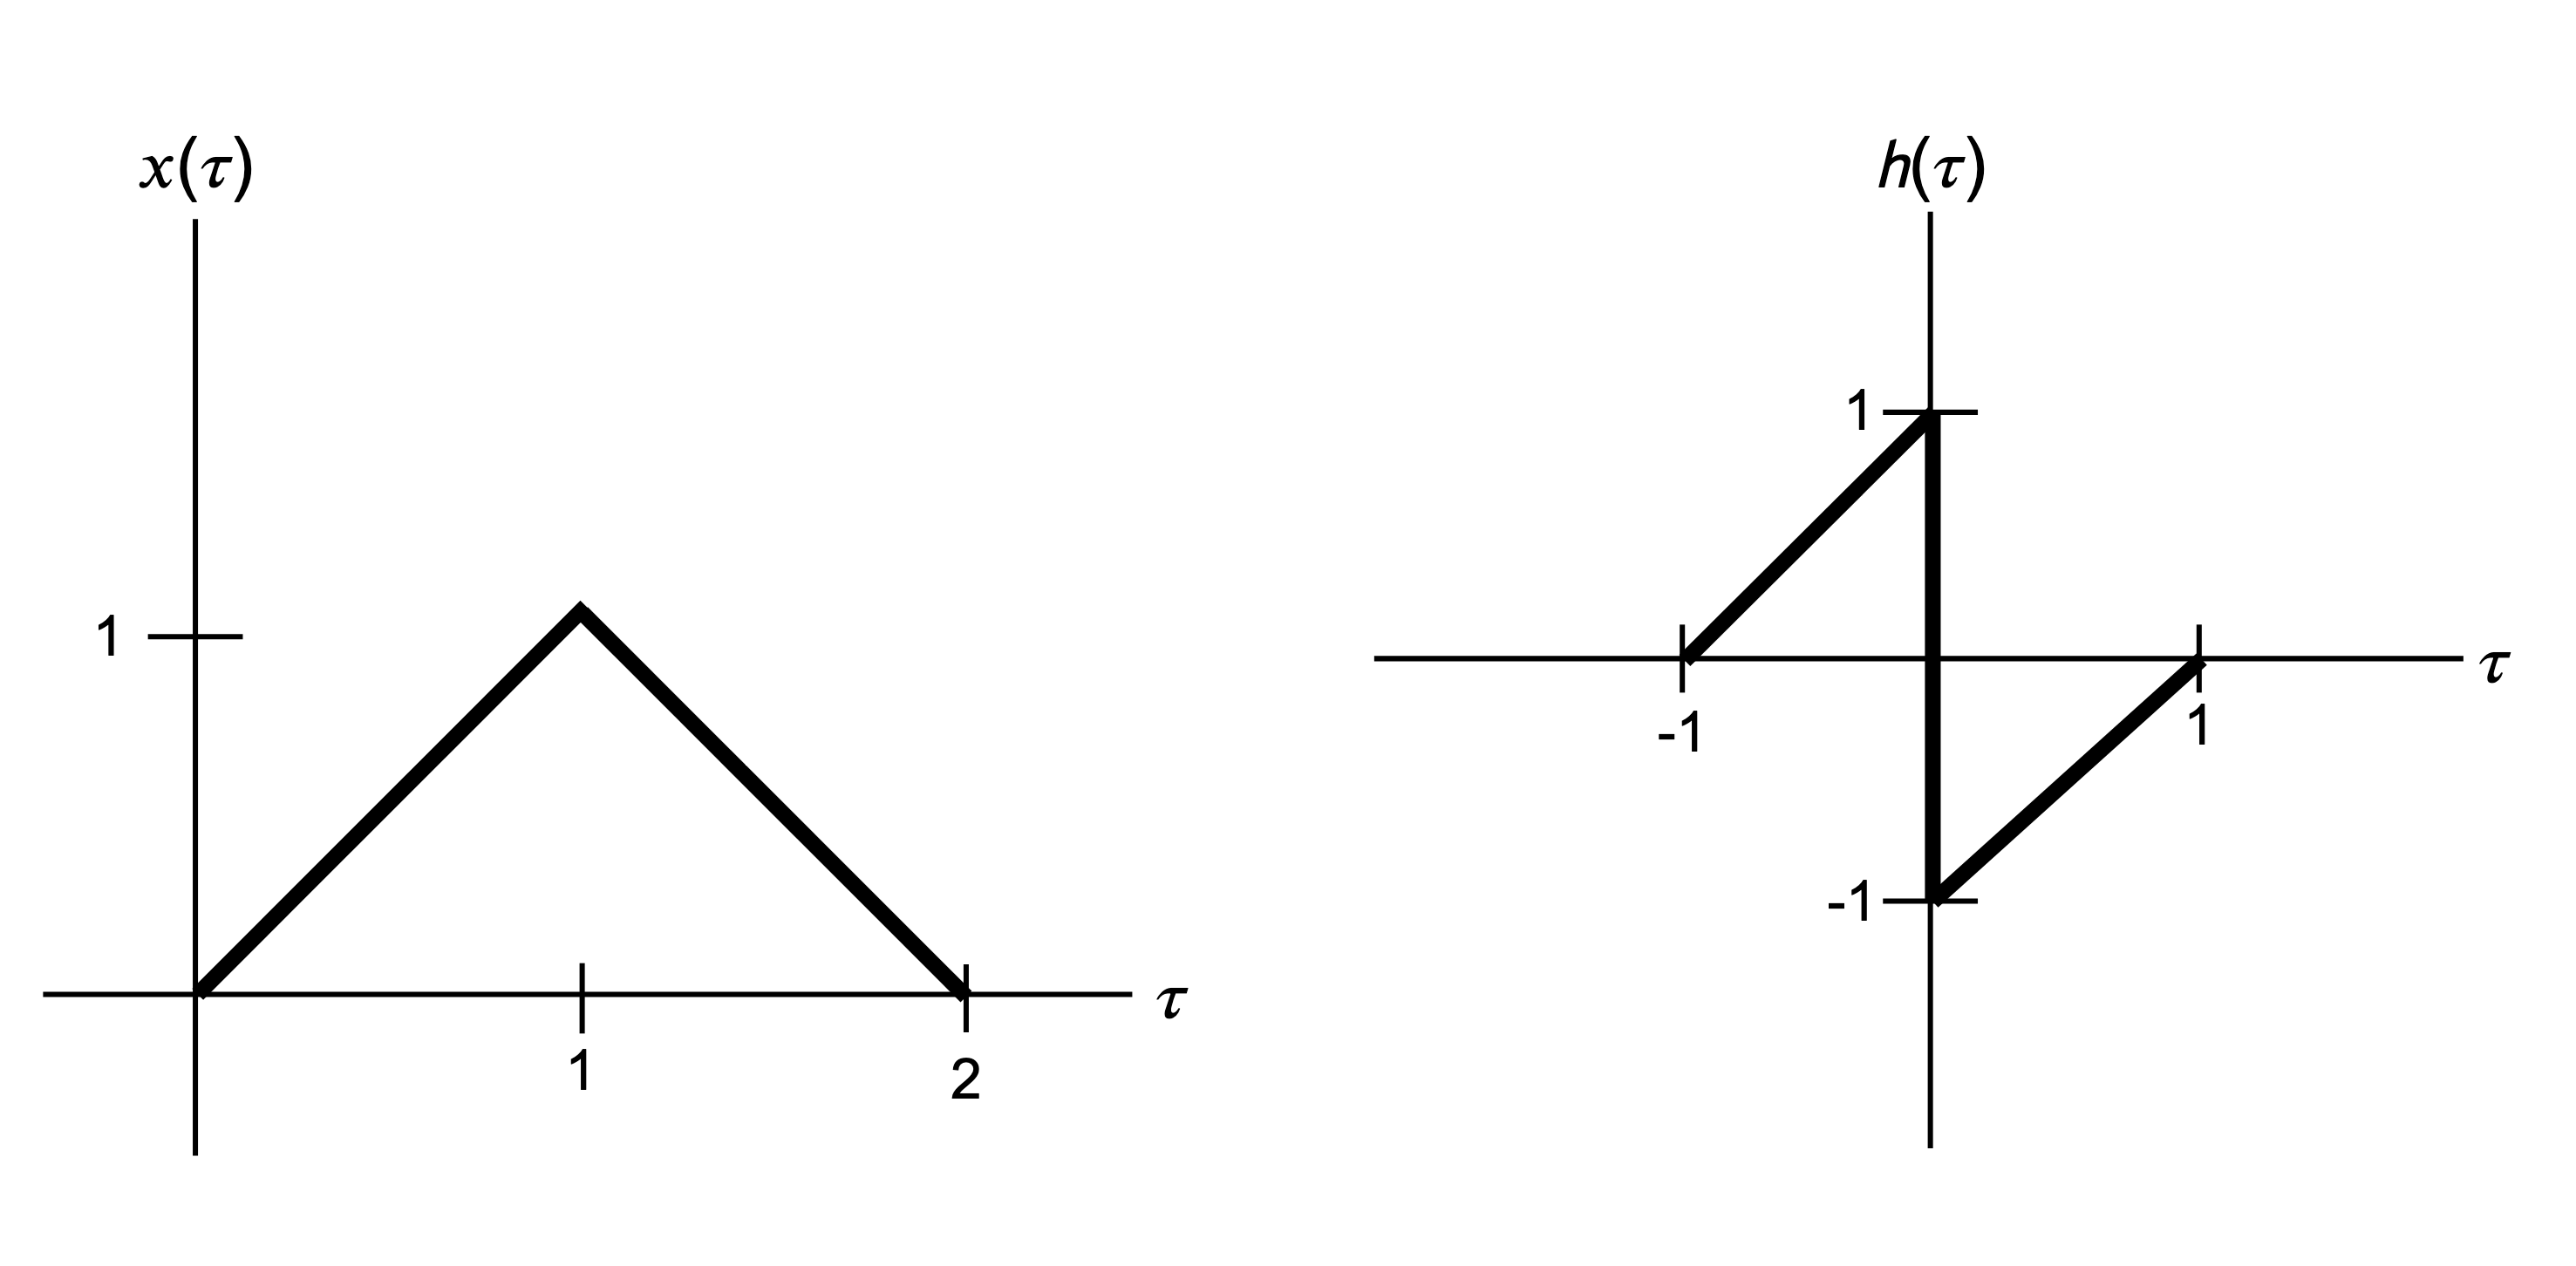
\includegraphics[width=0.9\textwidth]{41e1.png}
\end{center}
\begin{center}
    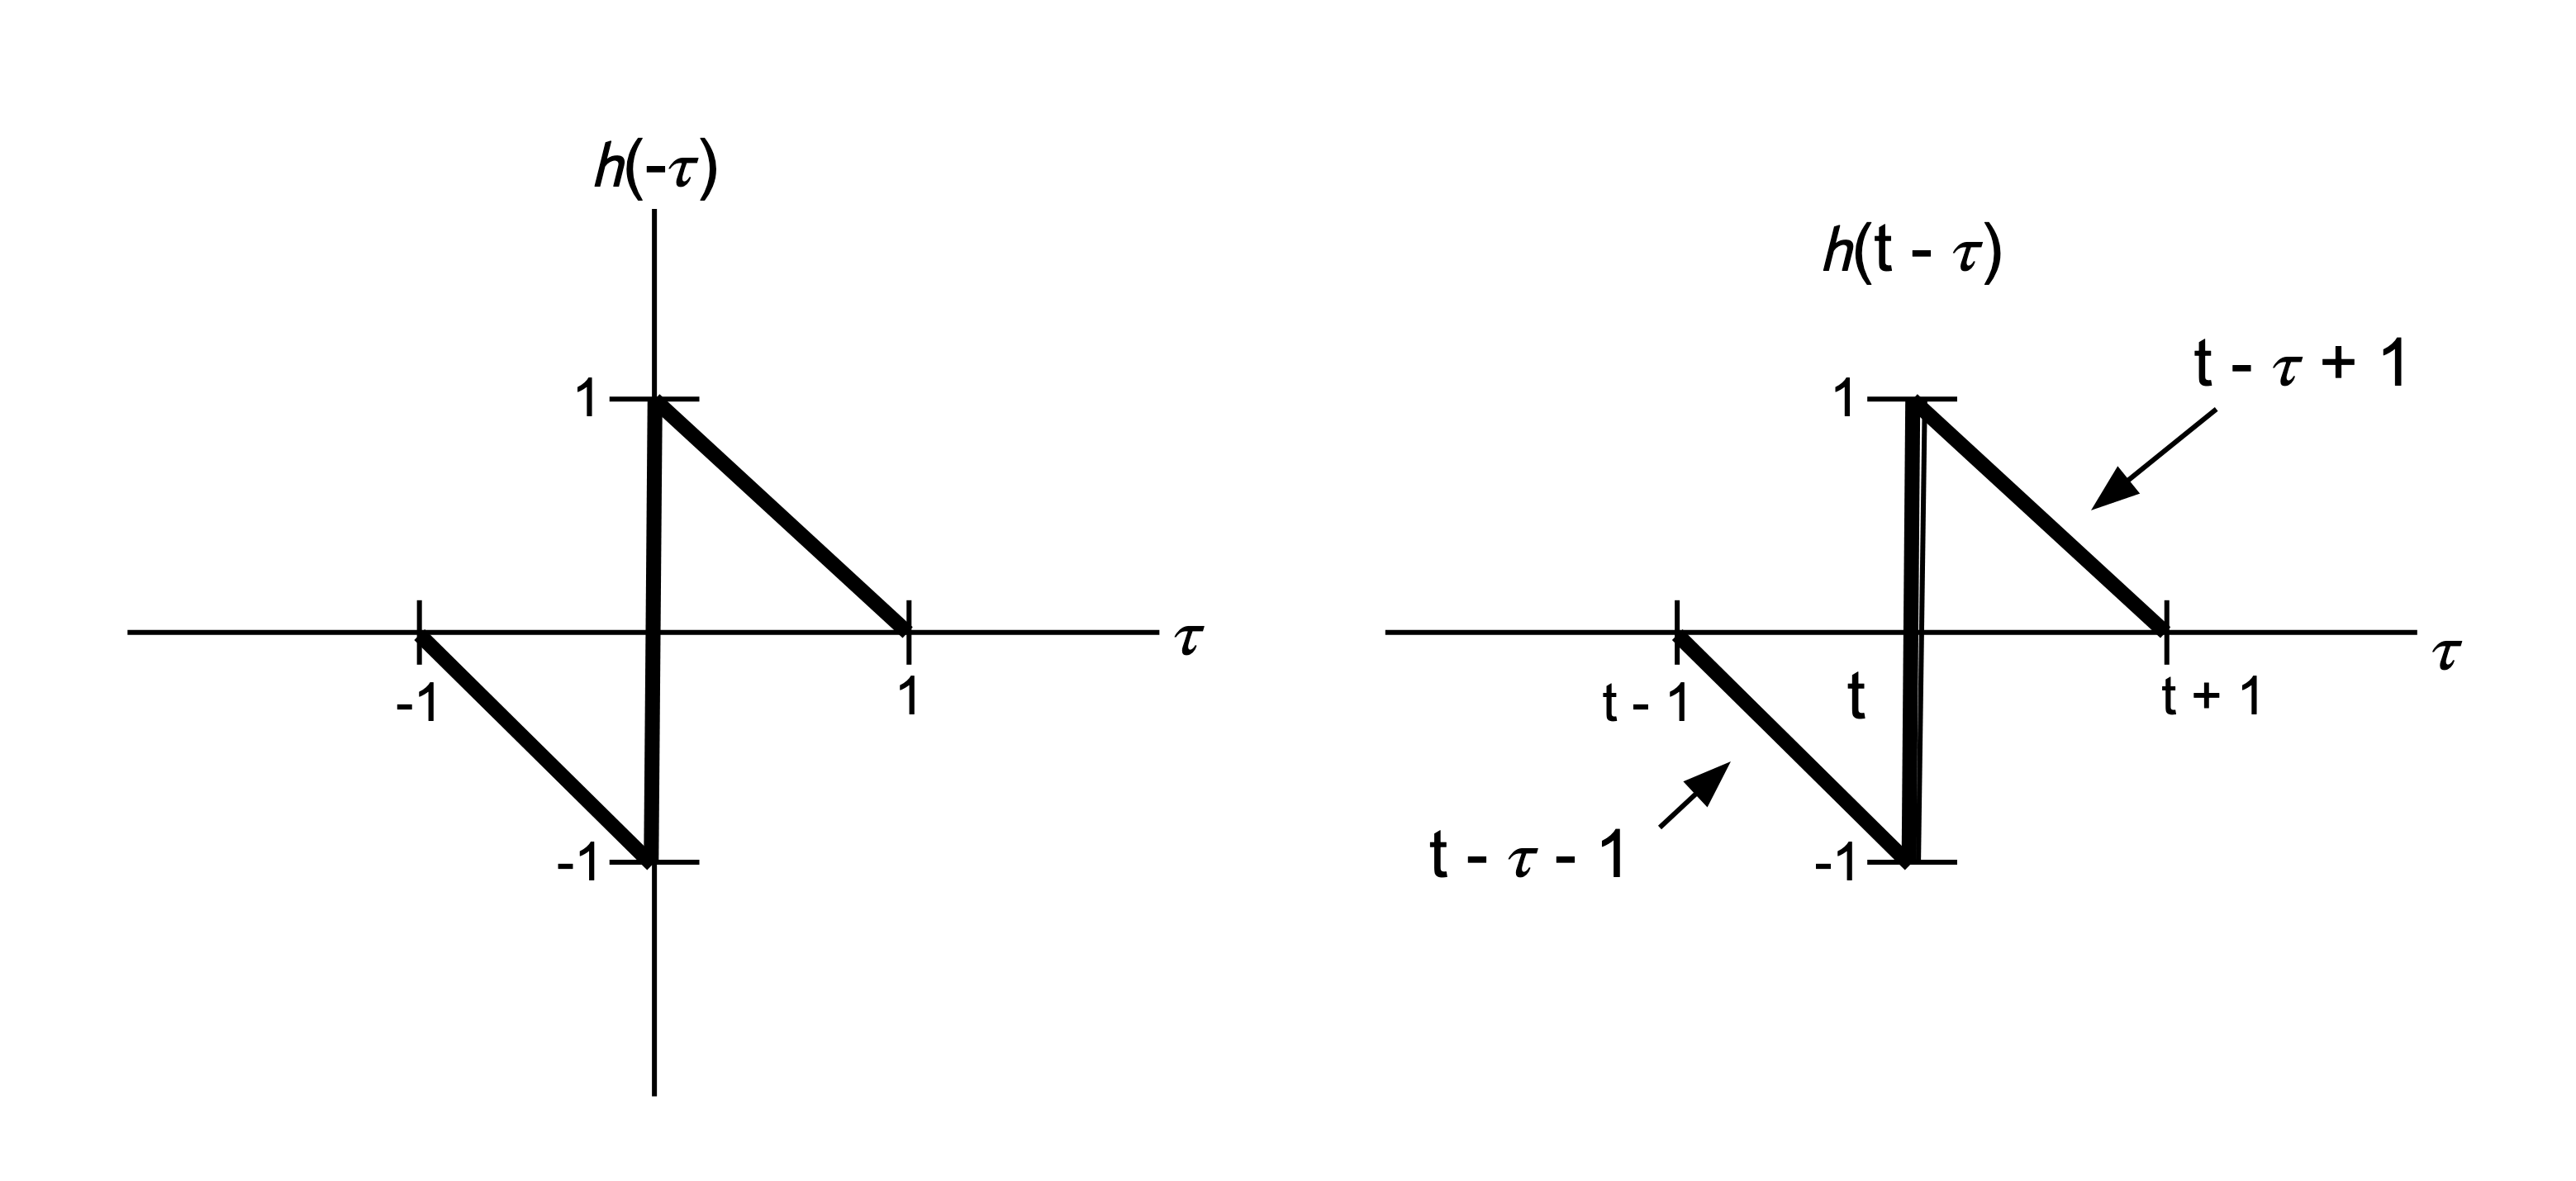
\includegraphics[width=0.9\textwidth]{41e2.png}
\end{center}
\begin{center}
    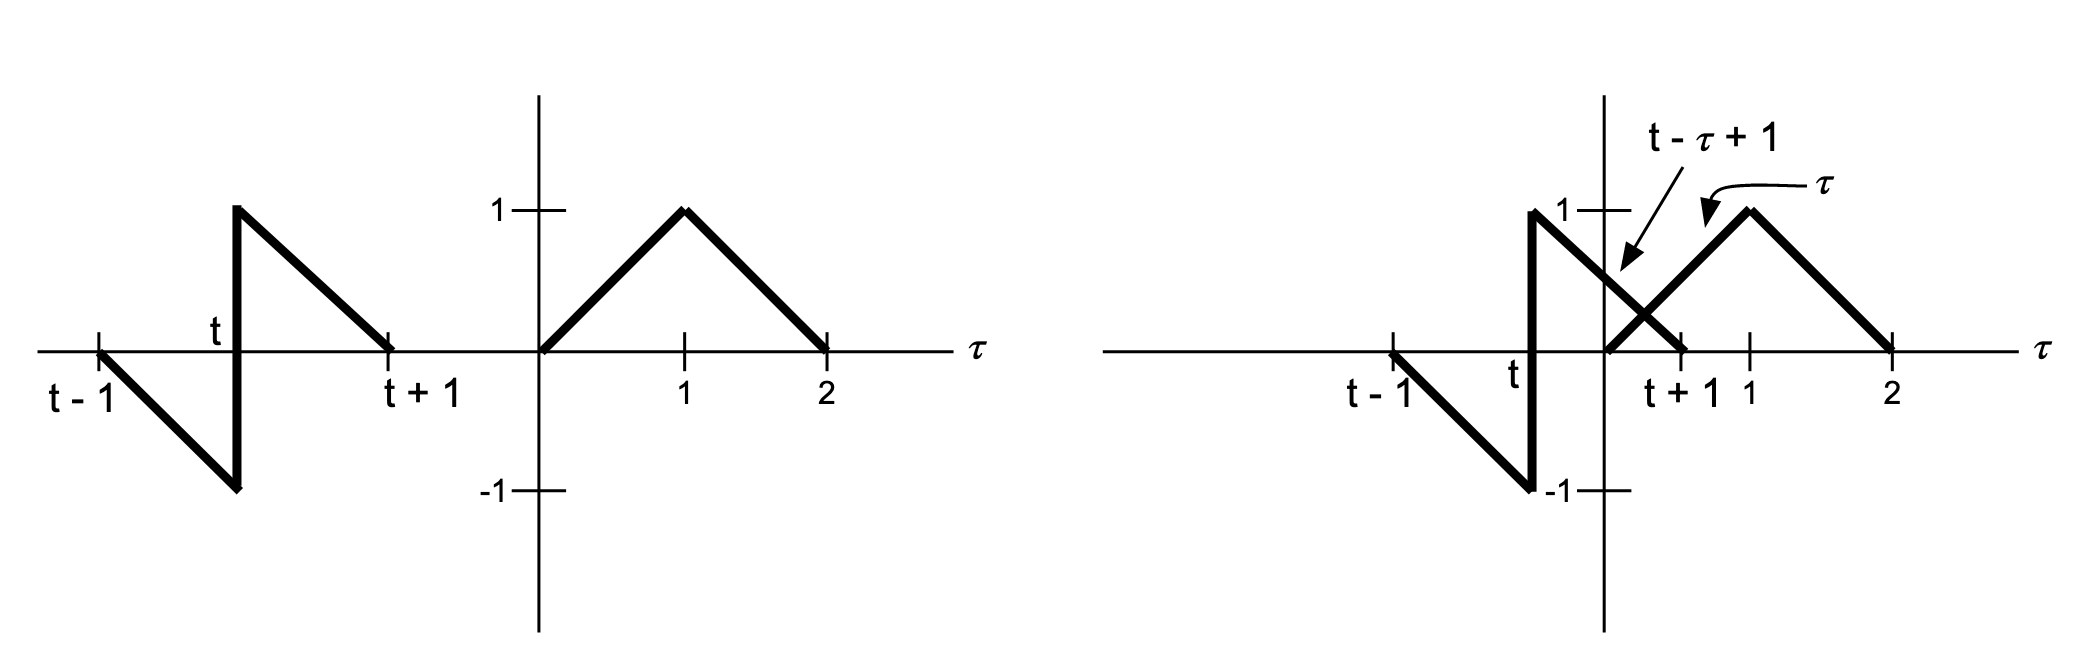
\includegraphics[width=0.9\textwidth]{41e3.png}
\end{center}
\begin{center}
    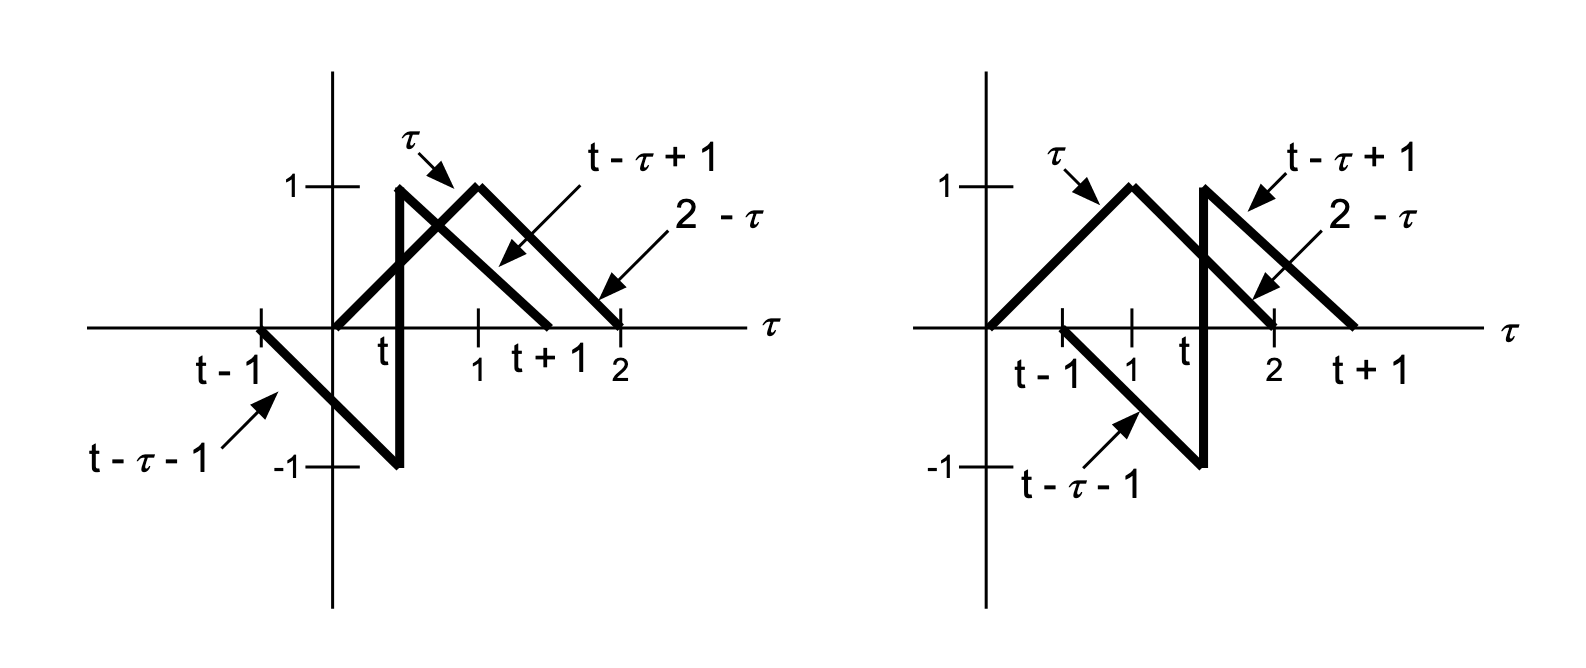
\includegraphics[width=0.9\textwidth]{41e4.png}
\end{center}
\begin{center}
    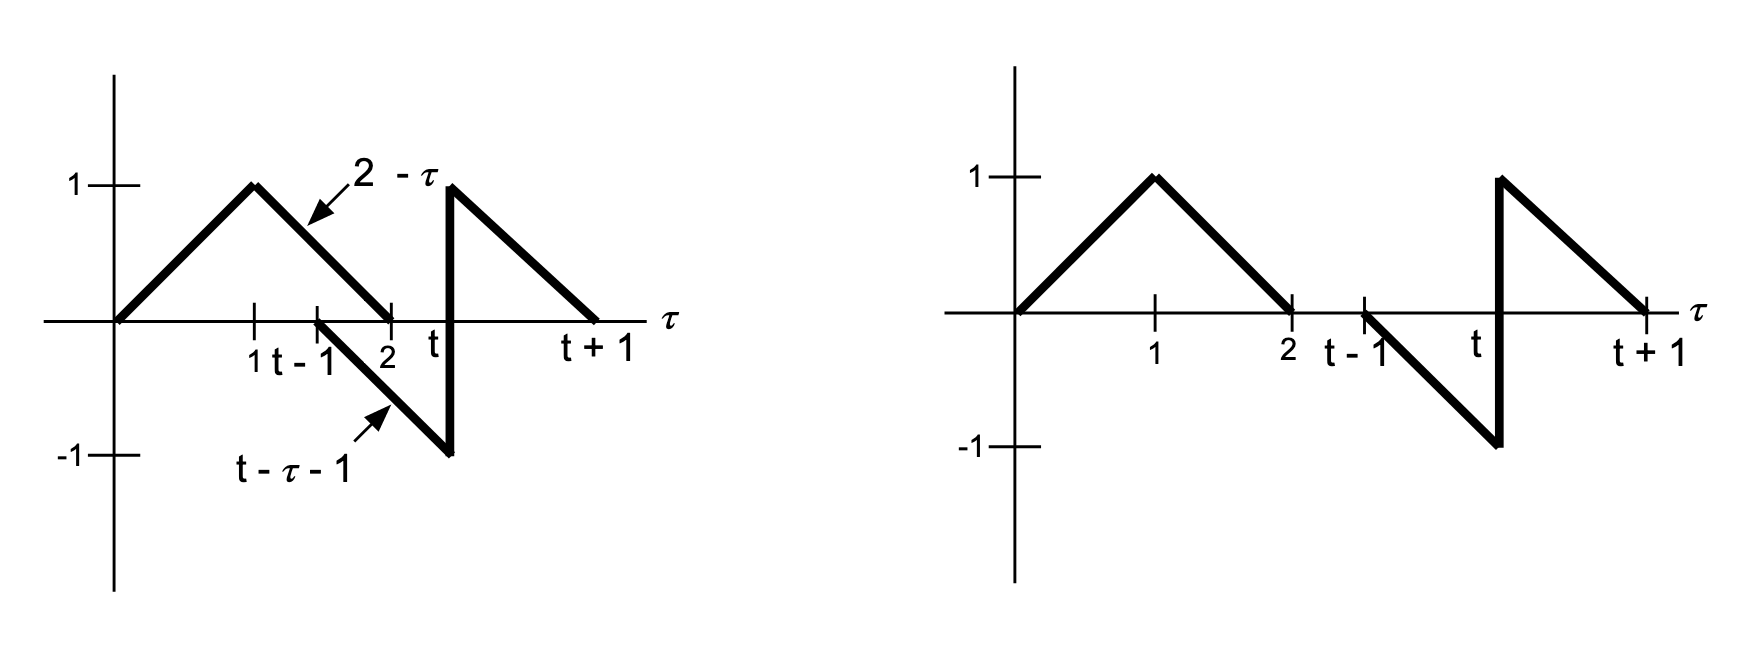
\includegraphics[width=0.9\textwidth]{41e5.png}
\end{center}

For the case of $t < -1$:
\begin{equation*}
\begin{split}
    x * h(t) = 0
\end{split}
\end{equation*}

For the case of $-1 \leq t < 1$:
\begin{equation*}
\begin{split}
    x * h(t) = \int_{0}^{t + 1} (\tau)(t - \tau + 1)d \tau
\end{split}
\end{equation*}

For the case of $0 \leq t < 1$:
\begin{equation*}
\begin{split}
    x * h(t) = \int_{0}^{t} (\tau)(t - \tau - 1)d \tau + \int_{t}^{1} (\tau)(t - \tau + 1)d \tau + \int_{1}^{t + 1} (2 - \tau)(t - \tau + 1)d \tau
\end{split}
\end{equation*}

For the case of $1 \leq t < 2$:
\begin{equation*}
\begin{split}
    x * h(t) = \int_{t-1}^{1} (\tau)(t - \tau - 1)d \tau + \int_{1}^{t} (2 - \tau)(t - \tau - 1)d \tau + \int_{t}^{2} (2 - \tau)(t - \tau + 1)d \tau
\end{split}
\end{equation*}

For the case of $2 \leq t < 3$:
\begin{equation*}
\begin{split}
    x * h(t) = \int_{t-1}^{2} (2 - \tau)(t - \tau - 1)d \tau
\end{split}
\end{equation*}

For the case of $t \geq 3$:
\begin{equation*}
\begin{split}
    x * h(t) = 0
\end{split}
\end{equation*}

Combining the above results we get:
\begin{equation*}
\begin{split}
    x * h(t)
    &= \begin{cases}
        \int_{0}^{t+1} (\tau) (t - \tau + 1)d\tau & -1 \leq t < 0\\
        \int_{0}^{t} (\tau)(t - \tau - 1)d \tau + \int_{t}^{1} (\tau)(t - \tau + 1)d \tau + \int_{1}^{t + 1} (2 - \tau)(t - \tau + 1)d \tau & 0 \leq t < 1\\
        \int_{t-1}^{1} (\tau)(t - \tau - 1)d \tau + \int_{1}^{t} (2 - \tau)(t - \tau - 1)d \tau + \int_{t}^{2} (2 - \tau)(t - \tau + 1)d \tau & 1 \leq t < 2\\
        \int_{t-1}^{2} (2 - \tau)(t - \tau - 1)d \tau & 2 \leq t < 3\\
        0 & otherwise
    \end{cases}\\
\end{split}
\end{equation*}


(f)
\begin{center}
    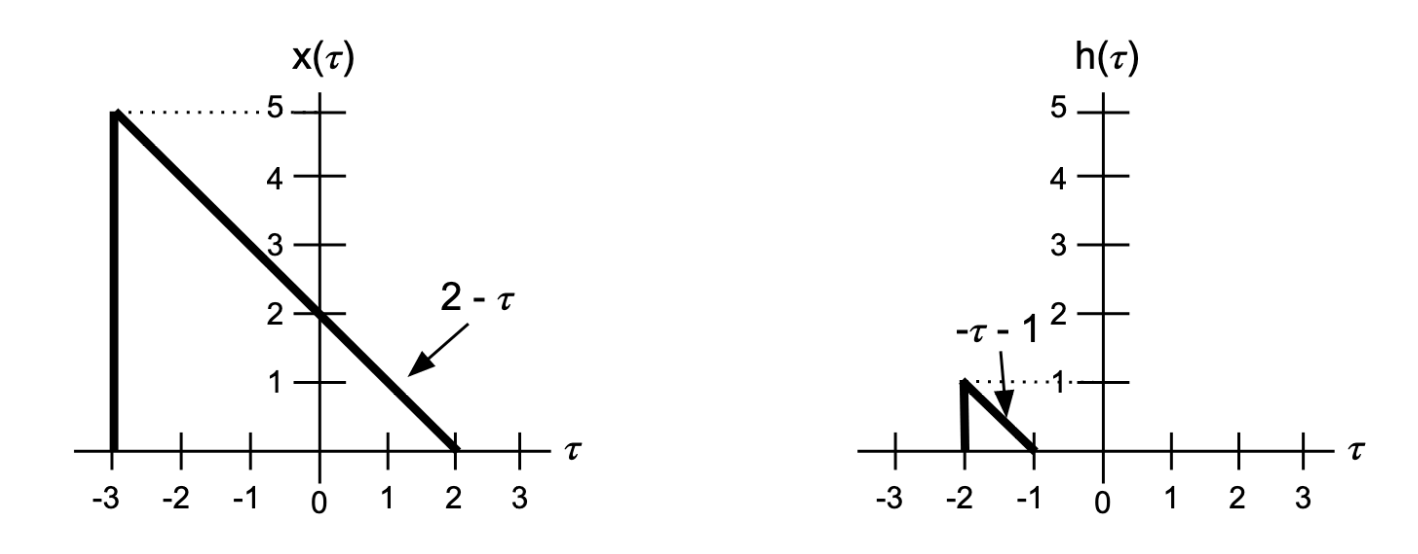
\includegraphics[width=0.9\textwidth]{41f1.png}
\end{center}
\begin{center}
    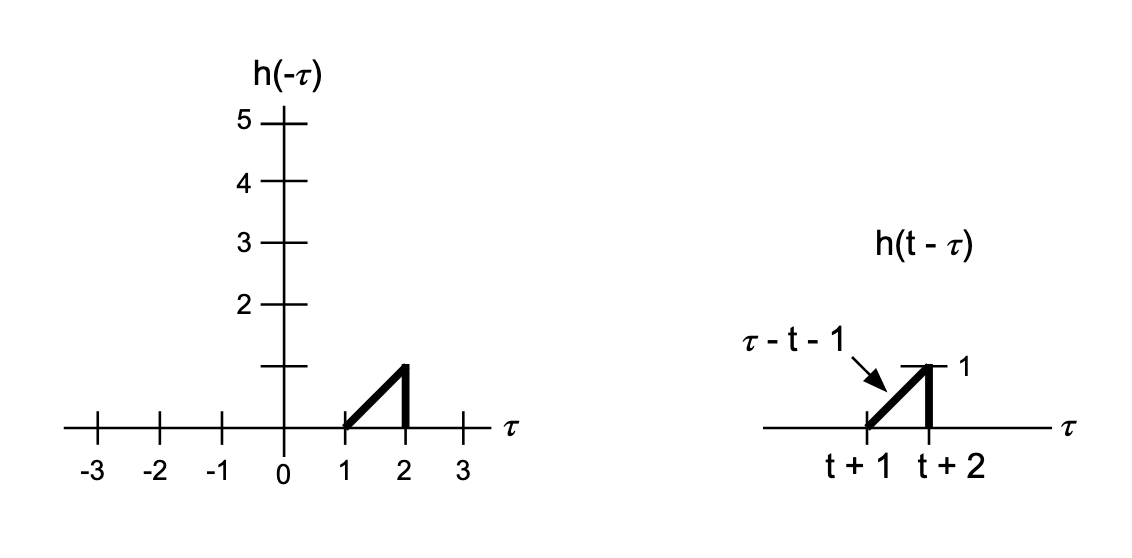
\includegraphics[width=0.9\textwidth]{41f2.png}
\end{center}
\begin{center}
    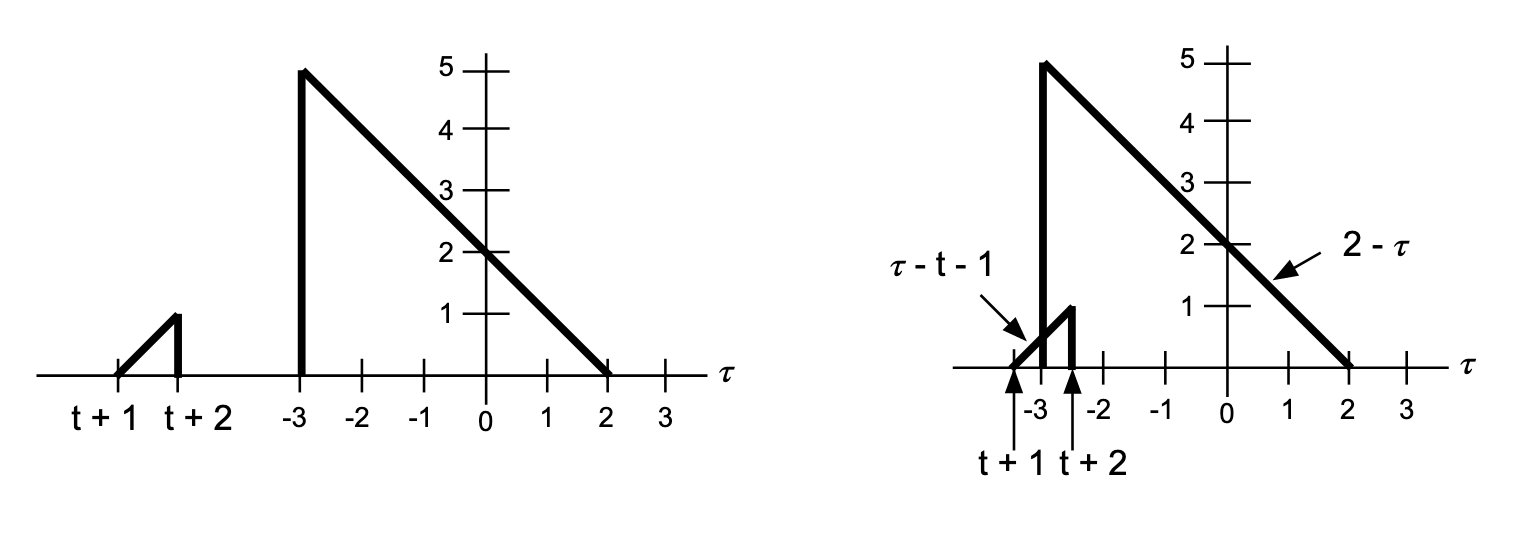
\includegraphics[width=0.9\textwidth]{41f3.png}
\end{center}
\begin{center}
    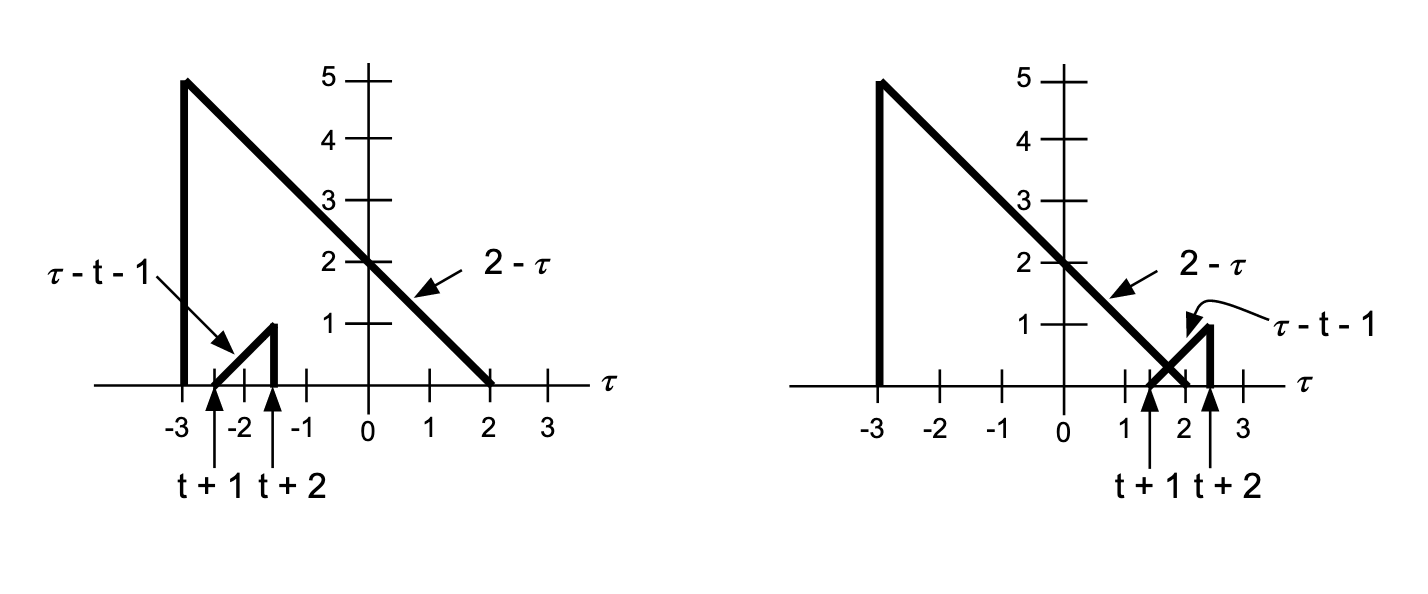
\includegraphics[width=0.9\textwidth]{41f4.png}
\end{center}
\begin{center}
    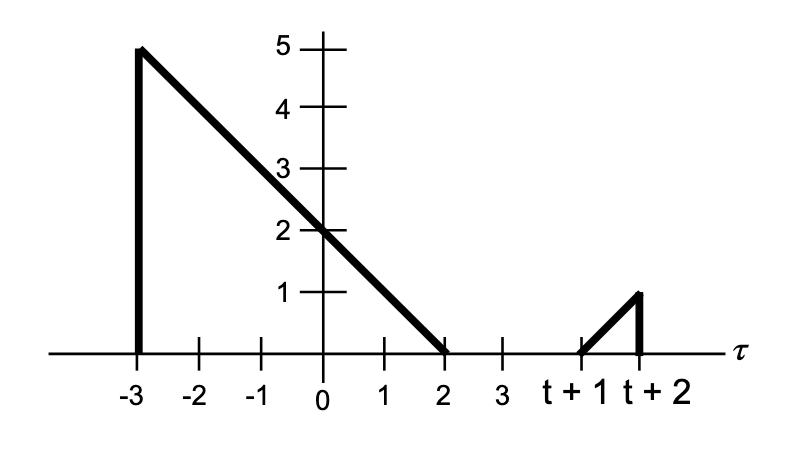
\includegraphics[width=0.5\textwidth]{41f5.png}
\end{center}

For the case of $t \leq -5$:
\begin{equation*}
\begin{split}
    x * h(t) = 0
\end{split}
\end{equation*}

For the case of $-5 \leq t < 4$:
\begin{equation*}
\begin{split}
    x * h(t) = \int_{-3}^{t + 2} (2 - \tau)(t - \tau - 1)d \tau
\end{split}
\end{equation*}

For the case of $-4 \leq t < 0$:
\begin{equation*}
\begin{split}
    x * h(t) = \int_{t + 1}^{t + 2} (2 - \tau)(t - \tau - 1)d \tau
\end{split}
\end{equation*}

For the case of $0 \leq t < 1$:
\begin{equation*}
\begin{split}
    x * h(t) = \int_{t + 1}^{2} (2 - \tau)(t - \tau - 1)d \tau
\end{split}
\end{equation*}

For the case of $t \geq 1$:
\begin{equation*}
\begin{split}
    x * h(t) = 0
\end{split}
\end{equation*}

Combining the above results we get:
\begin{equation*}
\begin{split}
    x * h(t)
    &= \begin{cases}
        \int_{-3}^{t + 2} (2 - \tau)(t - \tau - 1)d \tau & -5 \leq t < 4\\
        \int_{t + 1}^{t + 2} (2 - \tau)(t - \tau - 1)d \tau & -4 \leq t < 0\\
        \int_{t + 1}^{2} (2 - \tau)(t - \tau - 1)d \tau & 0 \leq t < 1\\
        0 & otherwise
    \end{cases}\\
\end{split}
\end{equation*}


\bigskip
4.3 {\bf [compute convolution]}\\
(b)
Using graphical method, we want to compute $x * h$ for each pair of function $x$ and $h$ for:
\begin{equation*}
\begin{split}
    x(t) = e^{-|t|} \text{ and } h(t) = rect(\frac{1}{3}[t - \frac{1}{2}])
\end{split}
\end{equation*}

\begin{center}
    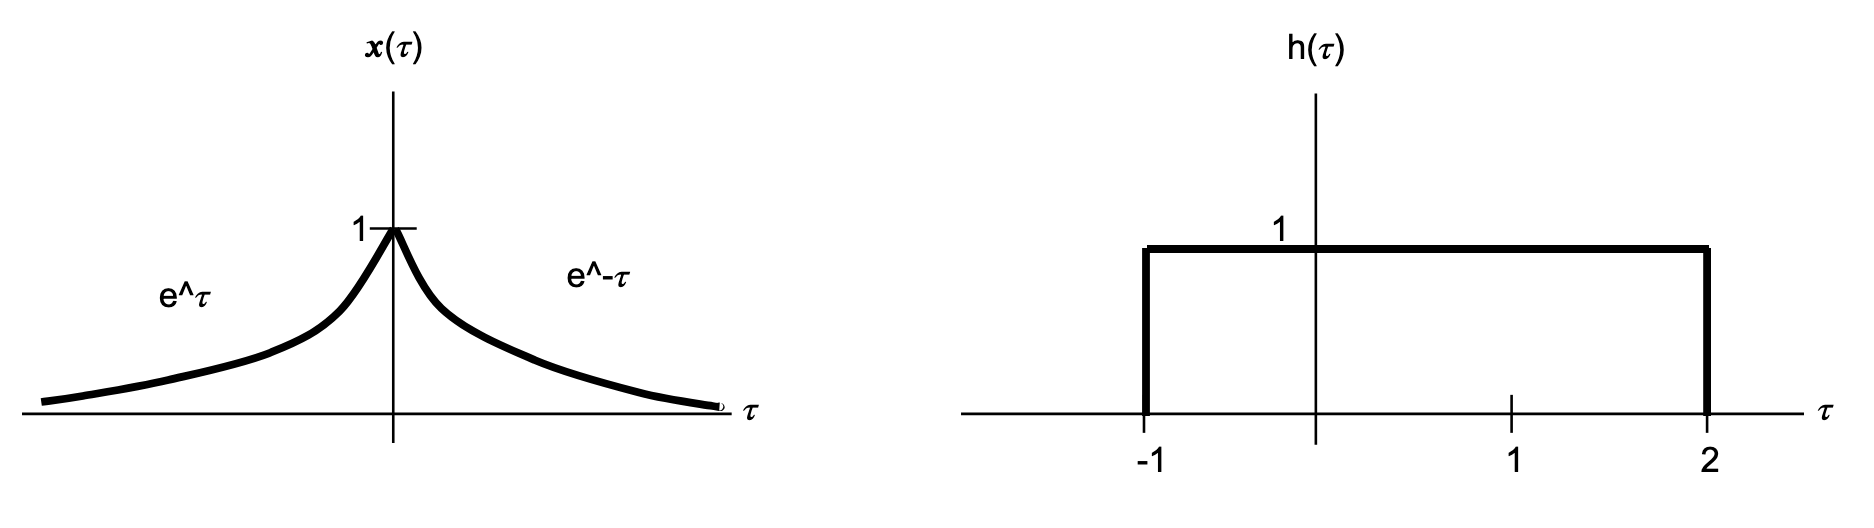
\includegraphics[width=0.9\textwidth]{43b1.png}
\end{center}
\begin{center}
    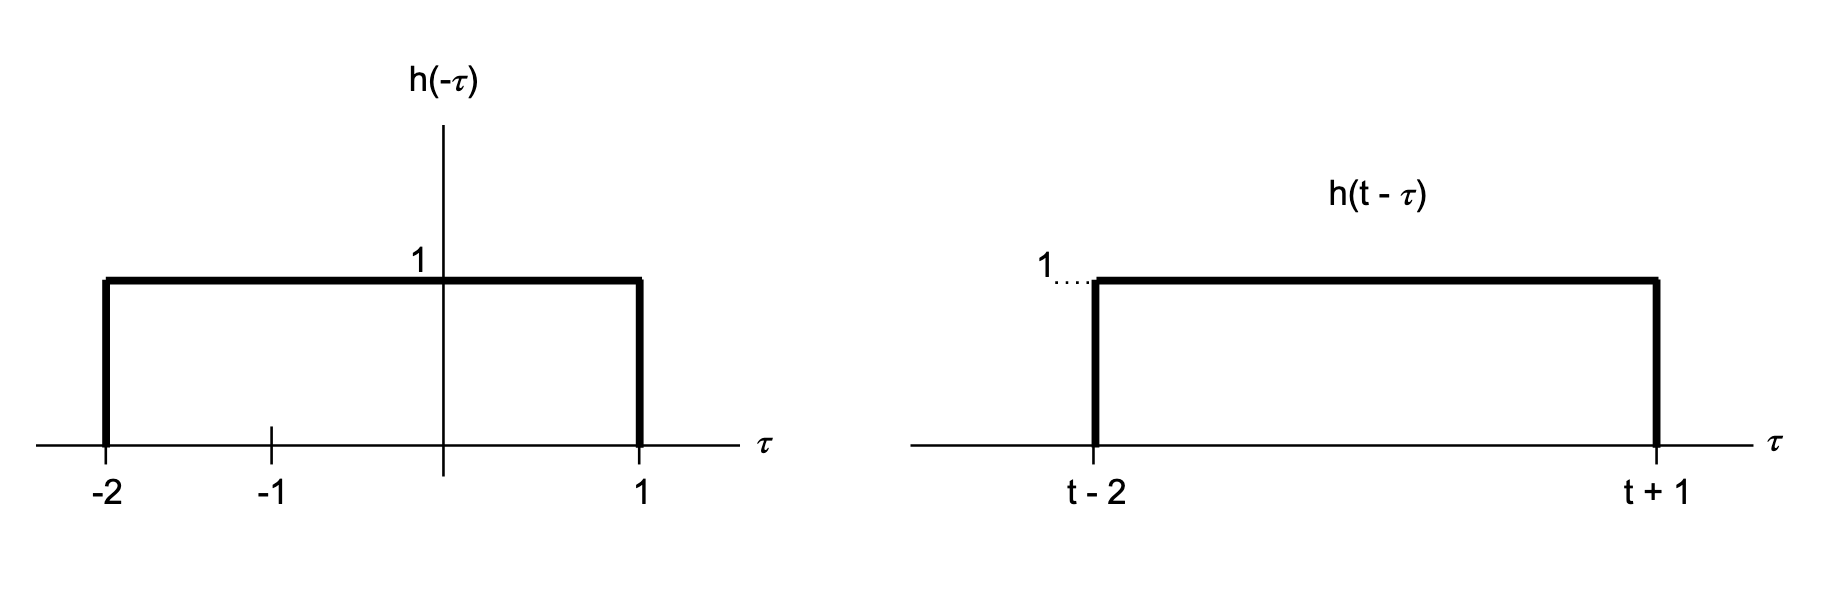
\includegraphics[width=0.9\textwidth]{43b2.png}
\end{center}
\begin{center}
    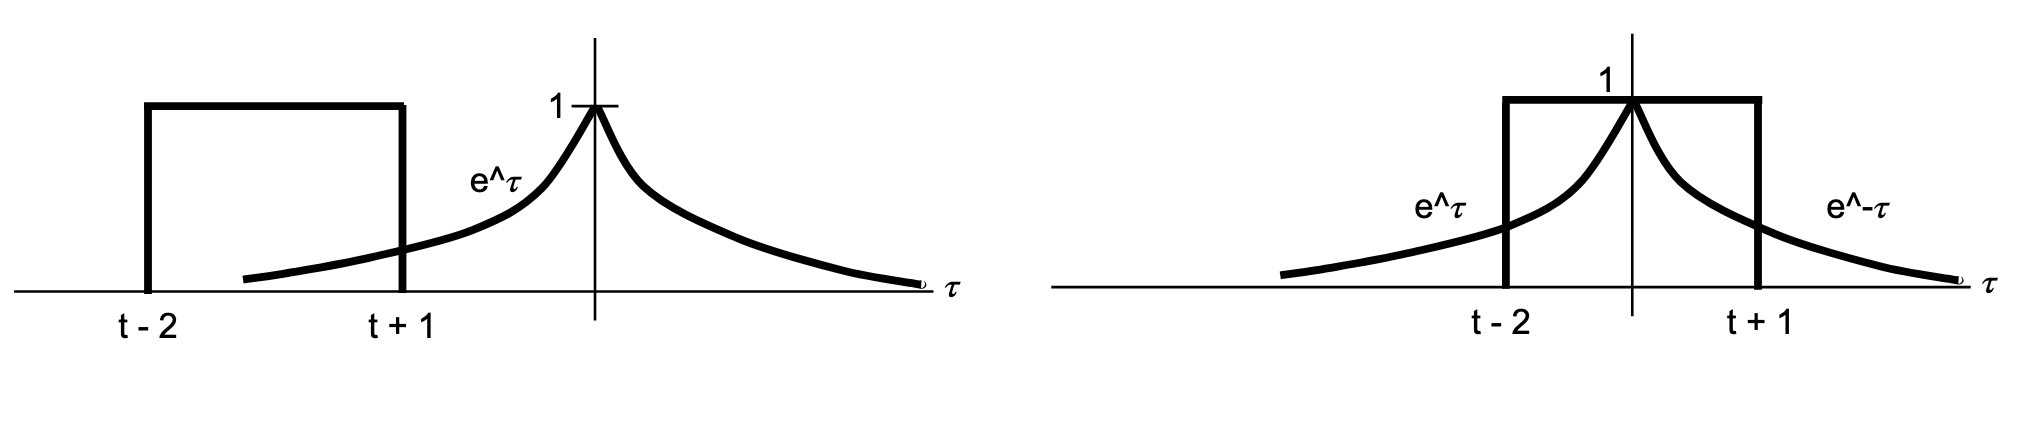
\includegraphics[width=0.9\textwidth]{43b3.png}
\end{center}
\begin{center}
    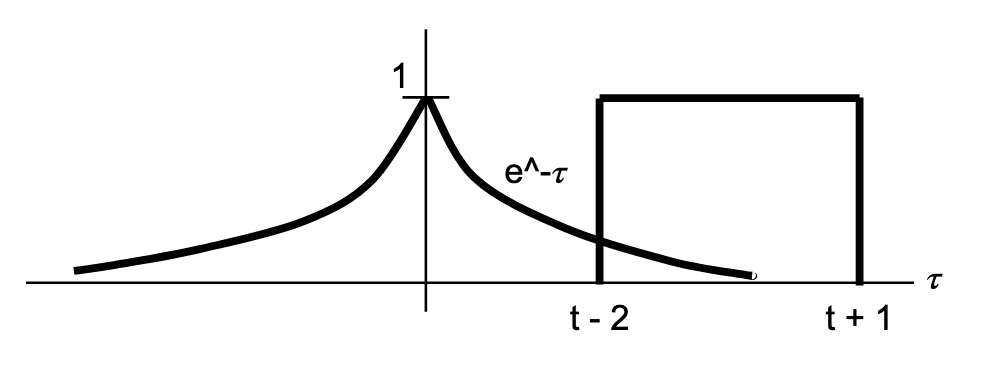
\includegraphics[width=0.5\textwidth]{43b4.png}
\end{center}

For the case of $t < -1$:
\begin{equation*}
\begin{split}
    x * h(t) = \int_{t - 2}^{t + 1}e^{\tau}d\tau
\end{split}
\end{equation*}

For the case of $-1 \leq t < 2$:
\begin{equation*}
\begin{split}
    x * h(t) = \int_{t - 2}^{0}e^{\tau}d\tau + \int_{0}^{t + 1}e^{-\tau}d\tau
\end{split}
\end{equation*}

For the case of $t \geq 2$:
\begin{equation*}
\begin{split}
    x * h(t) = \int_{t - 2}^{t + 1}e^{-\tau}d\tau
\end{split}
\end{equation*}

Combining the above results we get:
\begin{equation*}
\begin{split}
    x * h(t)
    &= \begin{cases}
        \int_{t - 2}^{t + 1}e^{\tau}d\tau & -1 \leq t < 2\\
        \int_{t - 2}^{0}e^{\tau}d\tau + \int_{0}^{t + 1}e^{-\tau}d\tau & -1 \leq t < 2\\
        \int_{t - 2}^{t + 1}e^{-\tau}d\tau & t \geq 2\\
    \end{cases}\\
\end{split}
\end{equation*}

(g)
\begin{center}
    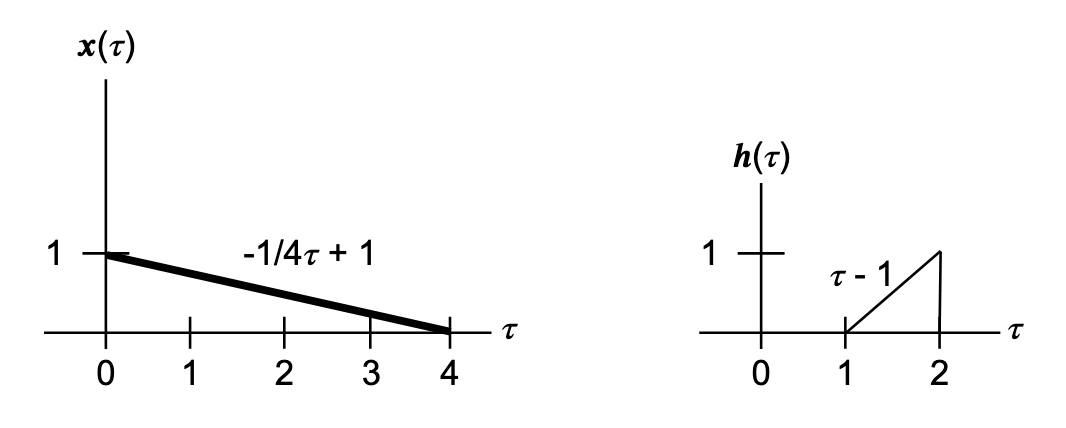
\includegraphics[width=0.8\textwidth]{43g1.png}
\end{center}
\begin{center}
    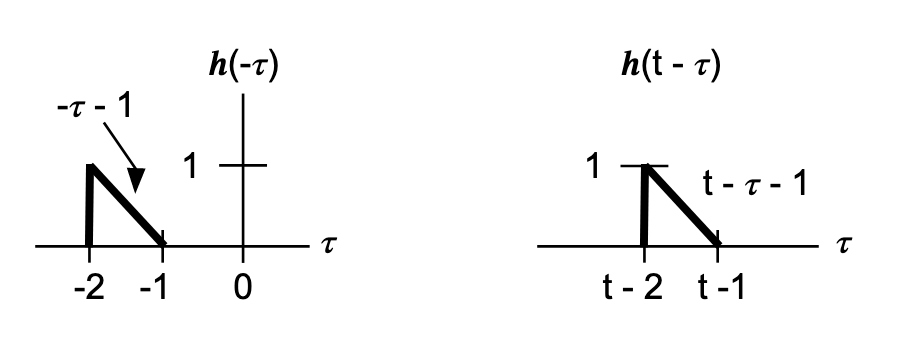
\includegraphics[width=0.8\textwidth]{43g2.png}
\end{center}
\begin{center}
    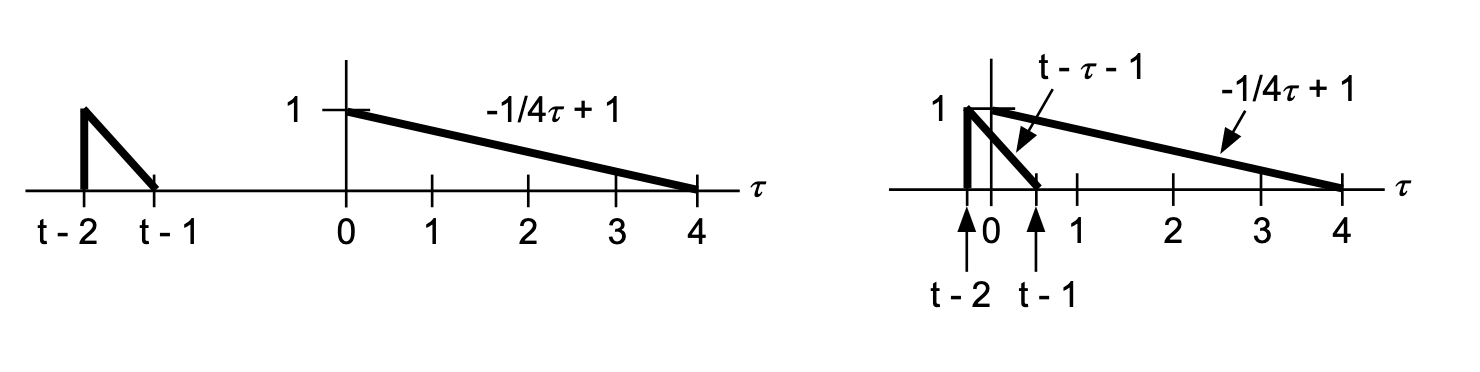
\includegraphics[width=0.8\textwidth]{43g3.png}
\end{center}
\begin{center}
    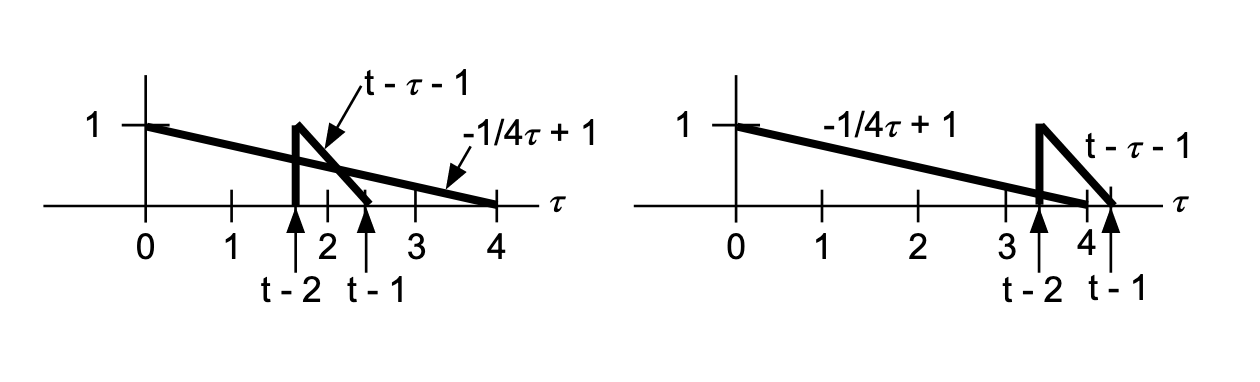
\includegraphics[width=0.8\textwidth]{43g4.png}
\end{center}
\begin{center}
    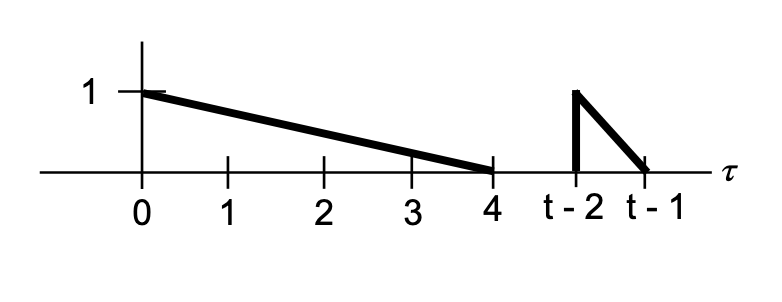
\includegraphics[width=0.5\textwidth]{43g5.png}
\end{center}

For the case of $t < 1$:
\begin{equation*}
\begin{split}
    x * h(t) = 0
\end{split}
\end{equation*}

For the case of $1 \leq t < 2$:
\begin{equation*}
\begin{split}
    x * h(t) = \int_{0}^{t - 1}(-\frac{1}{4}\tau + 1)(t - \tau - 1)d\tau
\end{split}
\end{equation*}

For the case of $2 \leq t < 5$:
\begin{equation*}
\begin{split}
    x * h(t) = \int_{t - 2}^{t - 1}(-\frac{1}{4}\tau + 1)(t - \tau - 1)d\tau
\end{split}
\end{equation*}

For the case of $5 \leq t < 6$:
\begin{equation*}
\begin{split}
    x * h(t) = \int_{t - 2}^{4}(-\frac{1}{4}\tau + 1)(t - \tau - 1)d\tau
\end{split}
\end{equation*}

For the case of $t \geq 6$:
\begin{equation*}
\begin{split}
    x * h(t) = 0
\end{split}
\end{equation*}

Combining the above results we get:
\begin{equation*}
\begin{split}
    x * h(t)
    &= \begin{cases}
        \int_{0}^{t - 1}(-\frac{1}{4}\tau + 1)(t - \tau - 1)d\tau & 1 \leq t < 2\\
        \int_{t - 2}^{t - 1}(-\frac{1}{4}\tau + 1)(t - \tau - 1)d\tau & 2 \leq t < 5\\
        \int_{t - 2}^{4}(-\frac{1}{4}\tau + 1)(t - \tau - 1)d\tau & 5 \leq t < 6\\
        0 & otherwise
    \end{cases}\\
\end{split}
\end{equation*}


\bigskip
{\bf 4.5 [manipulation of expressions involving convolution]}\\

Let $x,y,h$ and $v$ be function such that $y = x * h$ and
\begin{equation*}
\begin{split}
    v(t) = \int_{-\infty}^{\infty} x(-\tau - b)h(\tau + at)d\tau
\end{split}
\end{equation*}
where $a$ and $b$ are real constants. We want to express $v$ in terms of $y$.\\

Let $\delta = -\tau - b$, then $\tau = -\delta - b$ and $d\tau = -d\delta$

\begin{equation*}
\begin{split}
    v(t) &= \int_{-\infty}^{\infty} x(-\tau - b)h(\tau + at)d\tau\\
    &= \int_{\infty}^{-\infty} x(\delta)h((-\delta - b) + at) d\delta\\
    &= \int_{\infty}^{-\infty} x(\delta)h(at - b - \delta) d\delta\\
    &= y(at - b)
\end{split}
\end{equation*}


{\bf 4.6 [convolution property proof]}\\
(a)
Consider the convolution $y = x * h$. Assuming that he convolution $y$ exists, we want to prove that if $x$ is periodic, then $y$ is periodic.\\

If $x$ is periodic then $x(t) = x(t + T)$\\
Let $\delta = \tau + T$, and so $\tau = \delta - T$ and $d\delta = d\tau$

\begin{equation*}
\begin{split}
    y(t) &= \int_{-\infty}^{\infty} x(\tau)h(t - \tau)d\tau\\
    &= \int_{-\infty}^{\infty} x(\tau + T)h(t - \tau)d\tau\\
    &= \int_{-\infty}^{\infty} x(\delta - \tau + T)h(t - (\delta - T))d\delta\\
    &= \int_{-\infty}^{\infty} x(\delta)h(t - \delta + T)d\delta\\
    &= \int_{-\infty}^{\infty} x(\delta)h((t + T)- \delta)d\delta\\
    &= y(t + T)
\end{split}
\end{equation*}
$\therefore$ y is Periodic.


\bigskip
{\bf 4.9 [meaning of LTI]}\\
Consider a LTI system whose response to the function $x_1(t) = u(t) - u(t - 1)$ is the function $y_1$. We want to determine the response $y_2$ of the system to the input $x_2$ shown in the following figure in terms of $y_1$
\begin{center}
    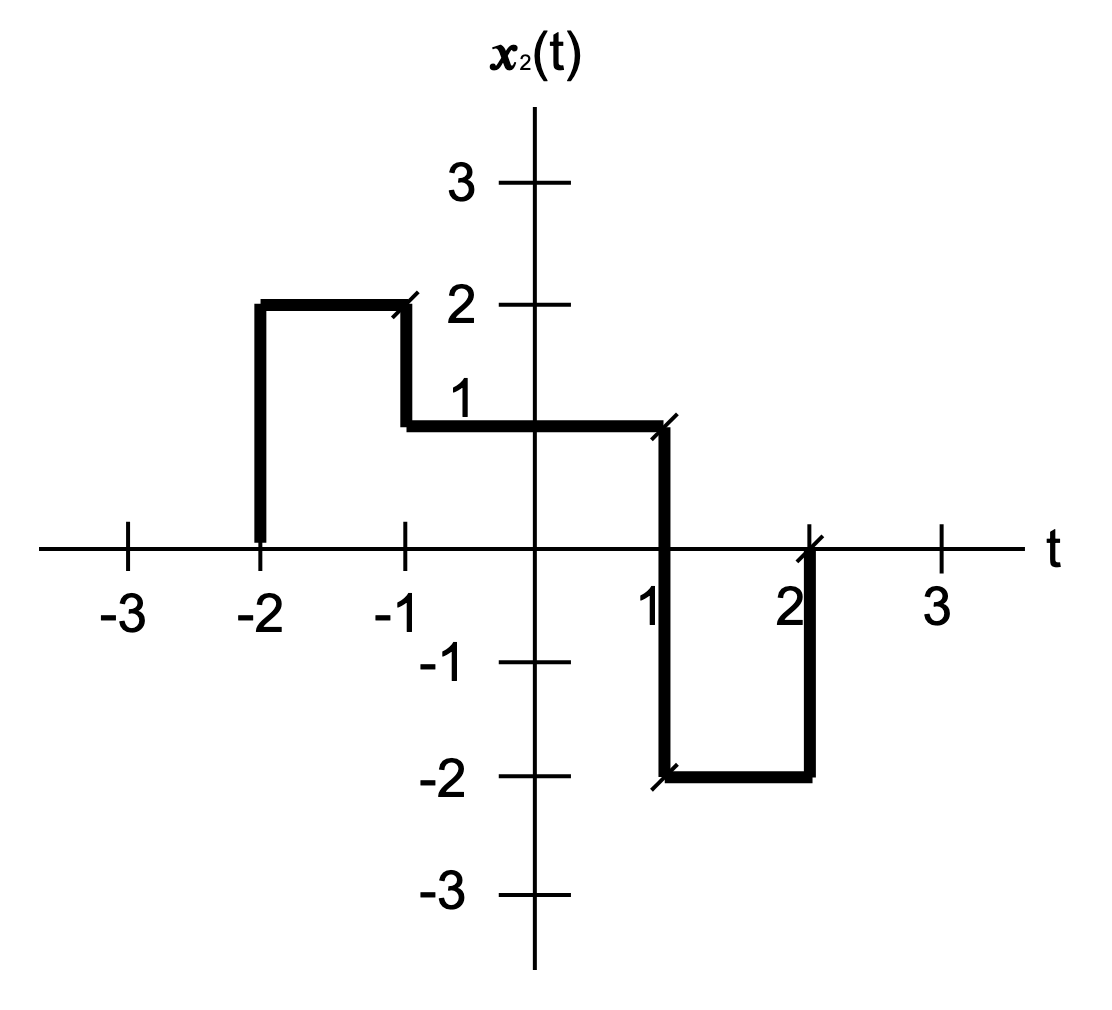
\includegraphics[width=0.5\textwidth]{49.png}
\end{center}

Since we know that $x_1(t) = u(t) - u(t - 1)$, we can represent $x_2$ in terms of $x_1$:
\begin{equation*}
\begin{split}
    v_1(t) &= 2u(t + 2)\\
    v_2(t) &= u(t + 1)\\
    v_3(t) &= u(t)\\
    v_4(t) &= 2u(t - 1)\\
    x_2(t) &= v_1(t) + v_2(t) + v_3(t) + v_4(t)\\\\
    x_2(t) &= 2u(t + 2) + u(t + 1) + u(t) - 2u(t - 1)
\end{split}
\end{equation*}

And so we can represent $x_2$ in terms of $x_1$ as follows:
\begin{equation*}
\begin{split}
    x_2(t) &= 2x_1(t + 2) + x_1(t + 1) + x_1(t) - 2x_1(t - 1)
\end{split}
\end{equation*}

Since it is an LTI system whose response to the function $x_1(t)$ is the function $y_1$, we get the following response:
\begin{equation*}
\begin{split}
    & 2y_1(t + 2) + y_1(t + 1) + y_1(t) - 2y_1(t - 1)\\
    \therefore \; & y_2(t) = 2y_1(t + 2) + y_1(t + 1) + y_1(t) - 2y_1(t - 1)
\end{split}
\end{equation*}


\bigskip
{\bf D.103 [plot, abds, angle, complex numbers]}\\
The following program and output plots $|F(\omega)|$ and $argF(\omega)$ for $\omega$ in the interval $[-10, 10]$, where $F$ denotes the complex-values function of a real variable given by:
\begin{equation*}
\begin{split}
    F(\omega) = \frac{1}{j \omega + 1}
\end{split}
\end{equation*}

\begin{lstlisting}
    w = linspace(-10, 10, 500);
    % f denotes the complex-values function of a real variable
    f = 1 ./ (j * w + 1);
    % Gets the phase angle
    fAngle = angle(f);
    % Gets the absolute value of f
    fAbs = abs(f);
    omeg = linspace(-10, 10, 500);
    % Plot arg(F(w))
    subplot(2, 1, 2);
    plot(omeg, fAngle);
    title('argF(\omega) for \omega in the interval [-10, 10]');
    xlabel('\omega');
    ylabel('argF(\omega)');
    % Plot |F(w)|
    subplot(2, 1, 1);
    plot(omeg, fAbs);
    title('|F(\omega)| for \omega in the interval [-10, 10]');
    xlabel('\omega');
    ylabel('|F(\omega)|');
\end{lstlisting}

\begin{center}
    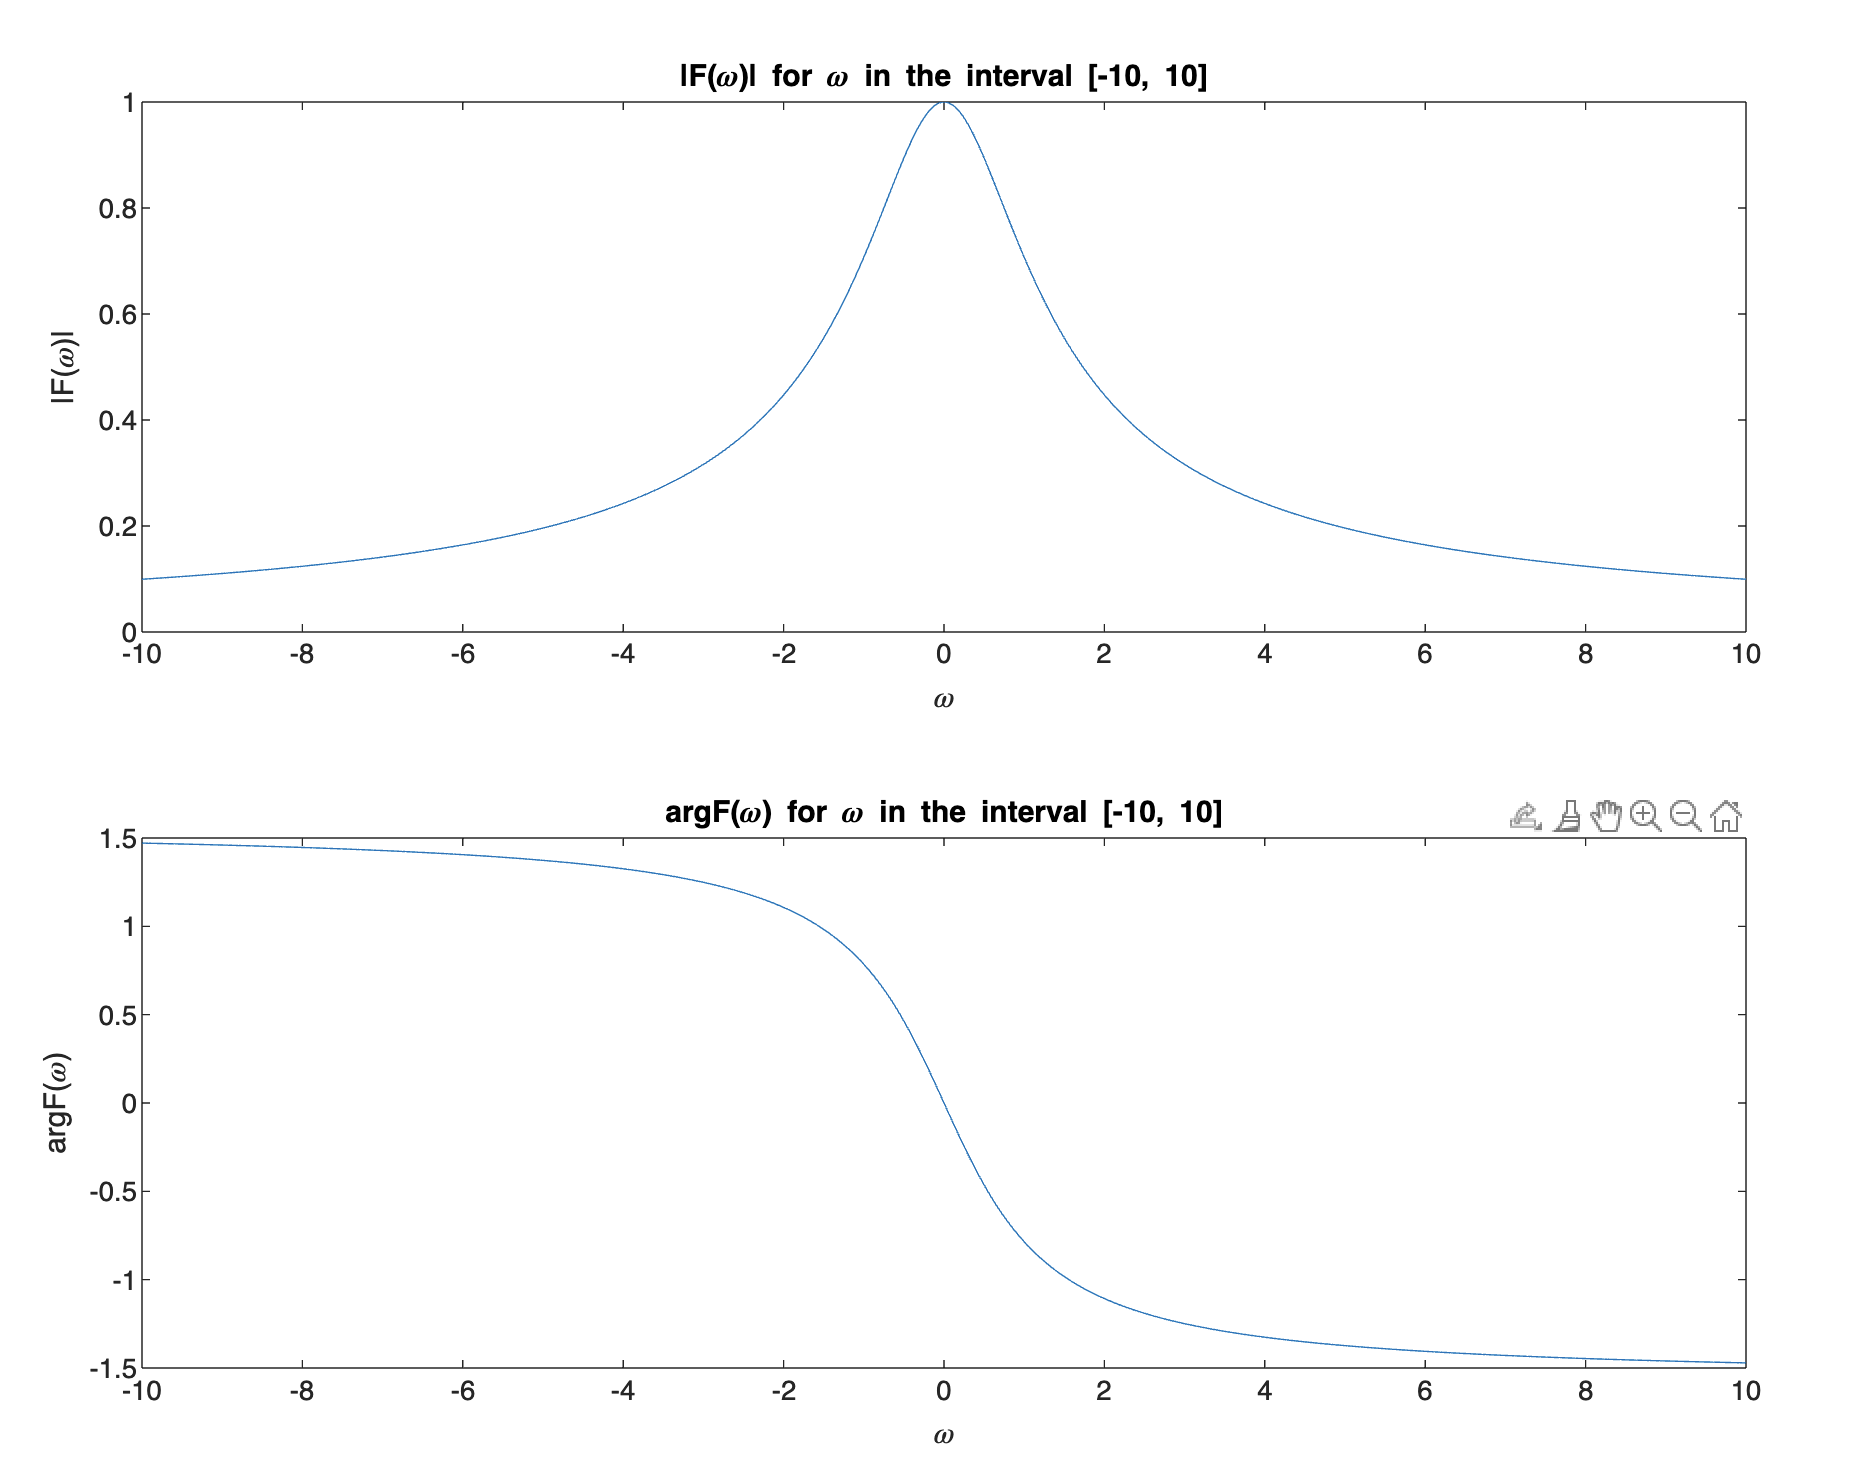
\includegraphics[width=1\textwidth]{103.png}
\end{center}


\end{document}
